\section{Activités d'enseignement}
\subsection{Dummy}
\begin{frame}{Actions collectives}
\begin{columns}
\begin{column}{0.6\textwidth}
\begin{block}{Responsabilités collectives}
\begin{itemize}
	\item Organisation des rencontres des jeunes physicien$\cdot$ne$\cdot$s
\end{itemize}
\end{block}
\begin{block}{Médiation \& vulgarisation scientifique}
\begin{itemize}
	\item Animation (Fête de la Science, Pint of Science)
	\item Ma thèse en 180 secondes
	\item Supports scientifiques (articles, vidéo)
\end{itemize}
\end{block}
\end{column}
\begin{column}{0.4\textwidth}
\centering
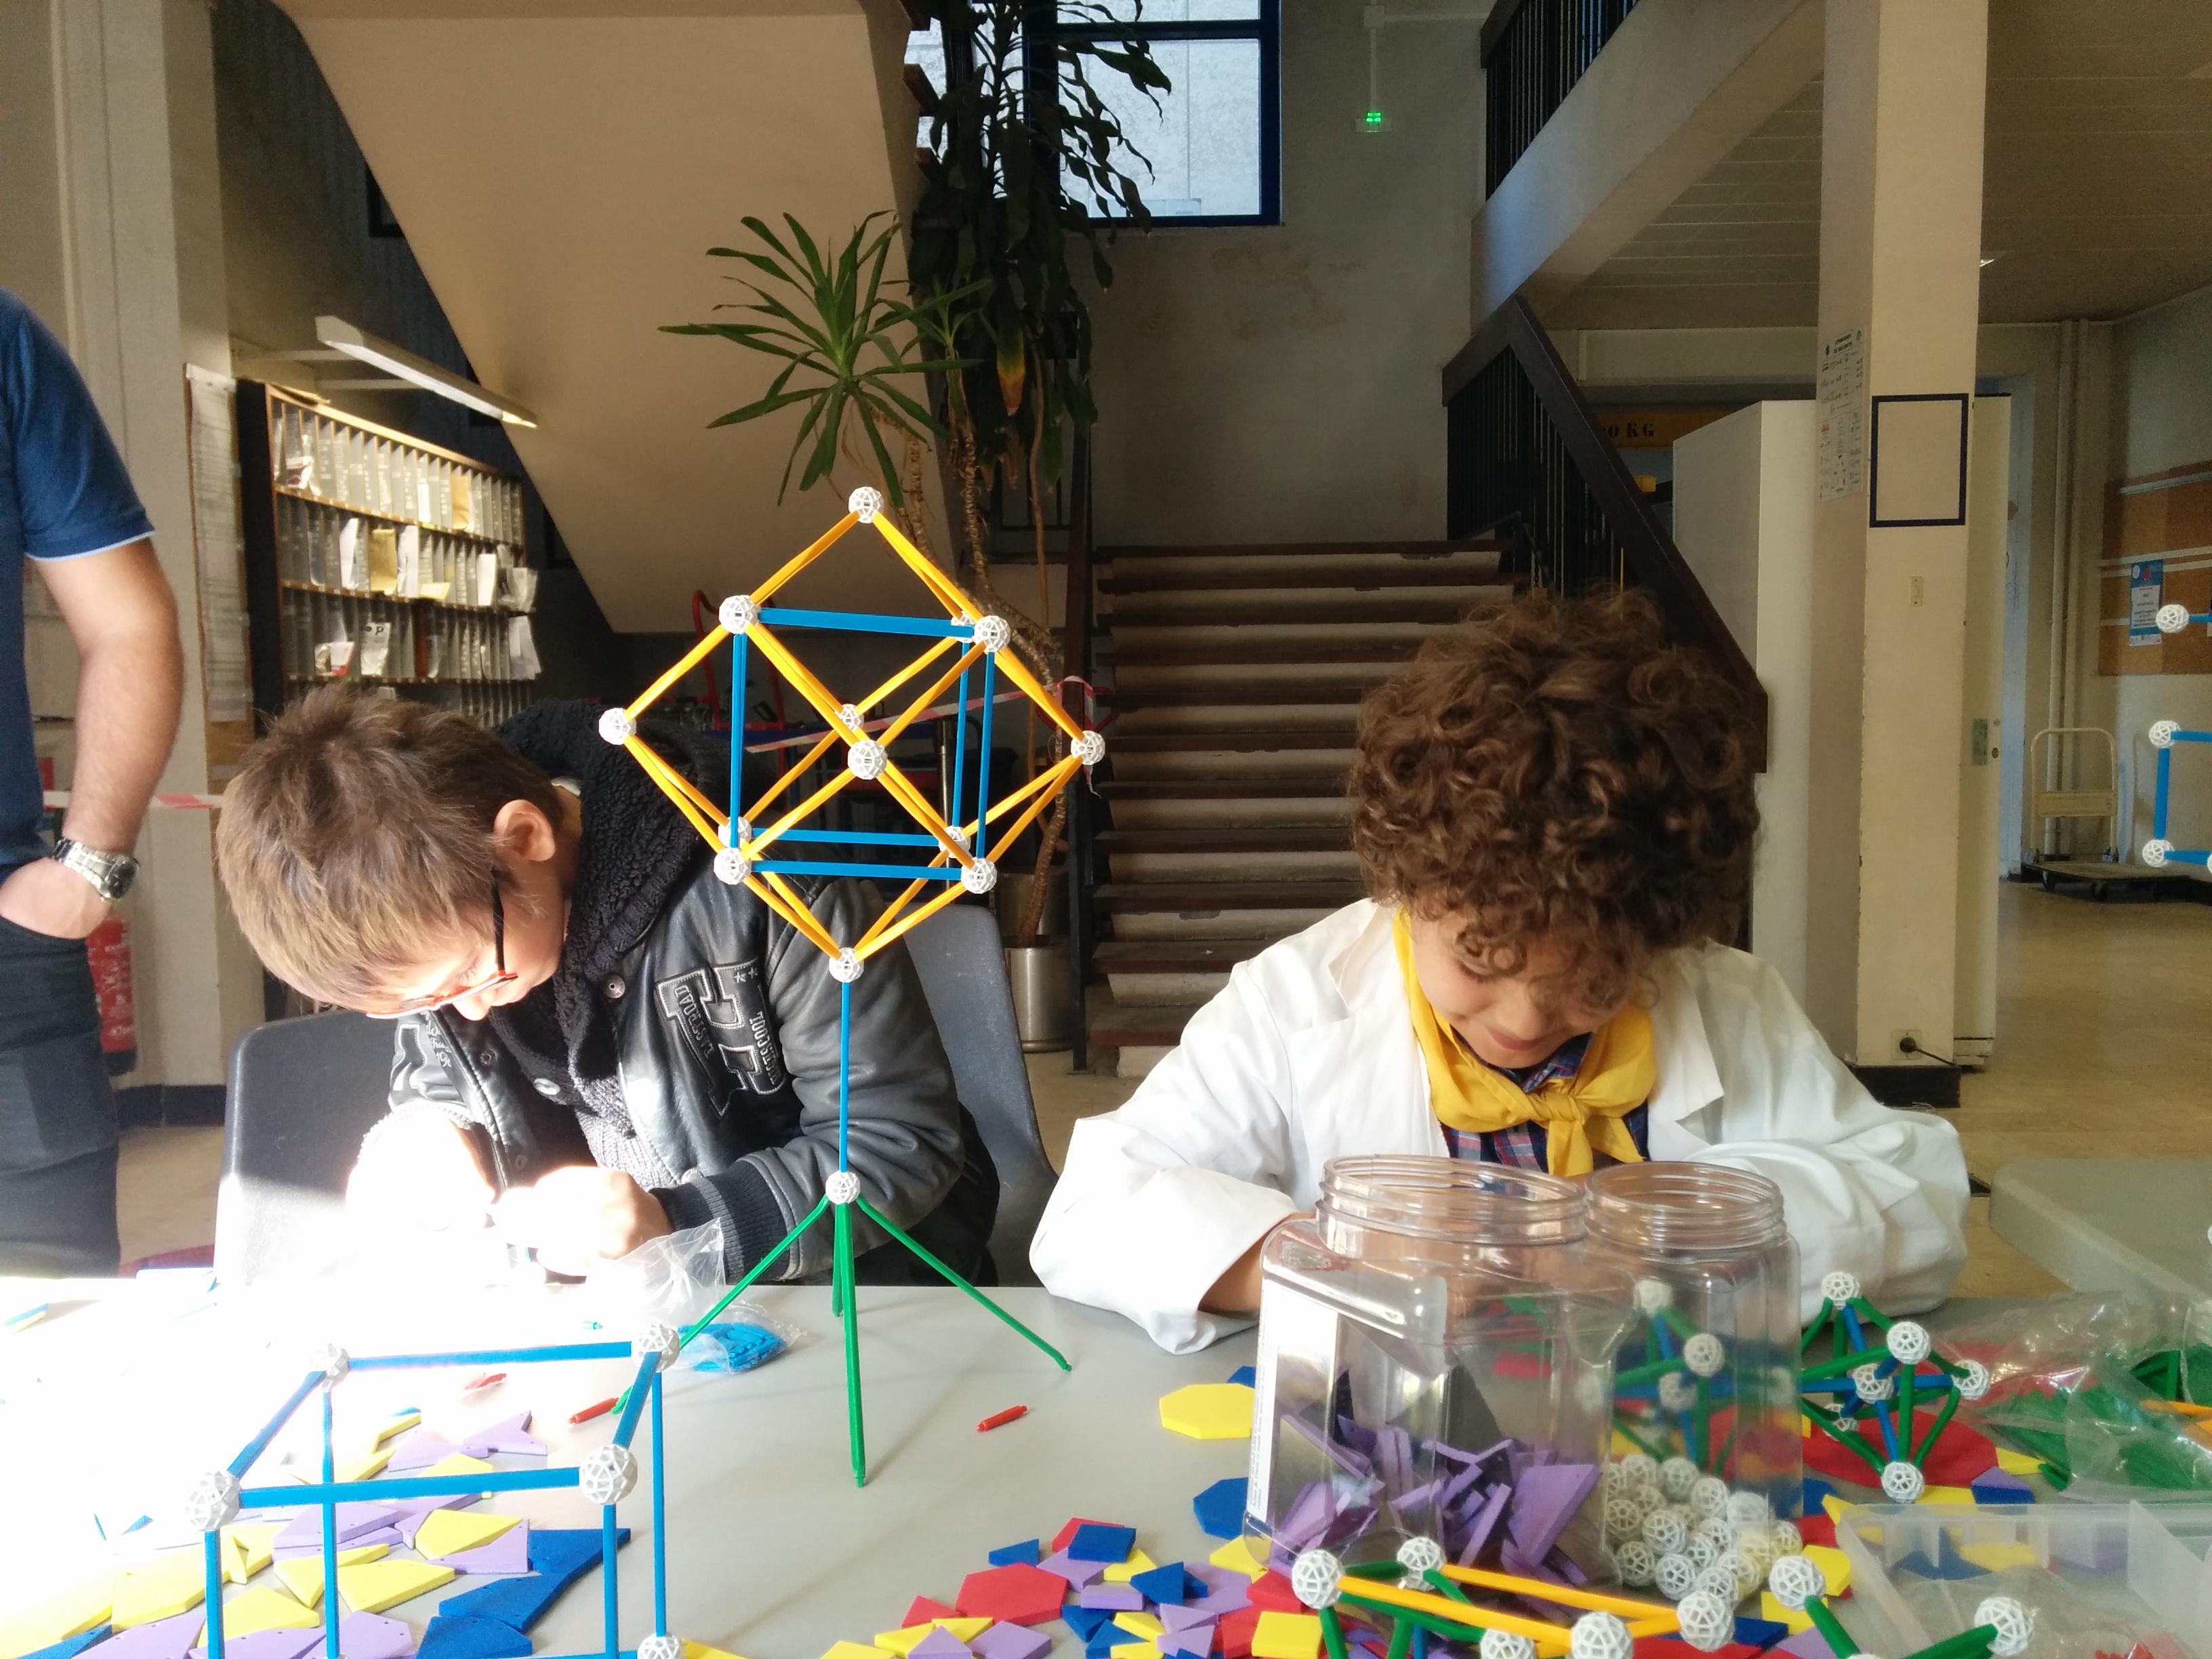
\includegraphics[width=\columnwidth]{img/3_projet_enseignement/fete_de_la_science}
\end{column}
\end{columns}
\end{frame}

\begin{frame}{Enseignement}
\begin{itemize}
	\item Tutorat de maths - L1 $\sim$ 20 h
	\item Optique géométrique (cours, TD, TP) - L1 $\sim$ 20 h
	\item Mécanique du solide \& physique des ondes (TD et TP) - L2 $\sim$ 160 h
	\item \textbf{Projet professionnel} - L1 $\sim$ 27 h
\end{itemize}
\end{frame}

\section{Projet d'enseignement}
\subsection{Dummy}
\begin{frame}{Séquence d'enseignement : Phénomènes ondulatoires -- L2, 60 heures}
Plan de cours :
\begin{columns}
	\begin{column}{0.5\textwidth}
		\begin{block}{\textbf{Ondes dans les milieux}}
			\begin{enumerate}
				\item Rappels : oscillateurs mécaniques,
				\item Cordes, ondes progressives,
				\item Ondes sonores, impédance,
				\item Ondes stationnaires, résonance.
			\end{enumerate}
		\end{block}
	\end{column}
	\begin{column}{0.5\textwidth}
		\begin{block}{\textbf{Optique ondulatoire}}
			\begin{enumerate}
				\item Ondes lumineuses,
				\item Interférences à deux ondes,
				\item Interférences à $N$ ondes,
				\item Polarisation.
			\end{enumerate}
		\end{block}
	\end{column}
\end{columns}
\begin{block}{\textbf{Défis}}
	\begin{itemize}
		\item Universalité des phénomènes ondulatoires $\to$ prise de recul
		\item Ondes lumineuses : évasives
	\end{itemize}
\end{block}
\end{frame}

\begin{frame}{La séquence en pratique}
\begin{block}{Fonctionnement en \textbf{classe inversée} :}
\begin{enumerate}
	\item \textbf{À la maison} ($\sim$ 4 h) : cours, exercices de compréhension (correction en ligne),
	\item \textbf{Cours} ($\sim$ 2 h) : applications directes, discussions,
	\item \textbf{TD} ($\sim$ 2 h) : travail d'approfondissement \textbf{en groupe},
	\item \textbf{TP} : 4 h, certaines semaines.
\end{enumerate}
\end{block}
\end{frame}

\begin{frame}{Une unité : Introduction aux interférences à deux ondes}
\begin{itemize}
	\item \textbf{À la maison} : conditions des interférences, interférences constructives/destructives, franges, etc.
	\item \textbf{En classe} : deux ondes planes, manip : cuve à ondes.
	\item \textbf{TD numérique} : deux ondes cylindriques.
\end{itemize}
\centering
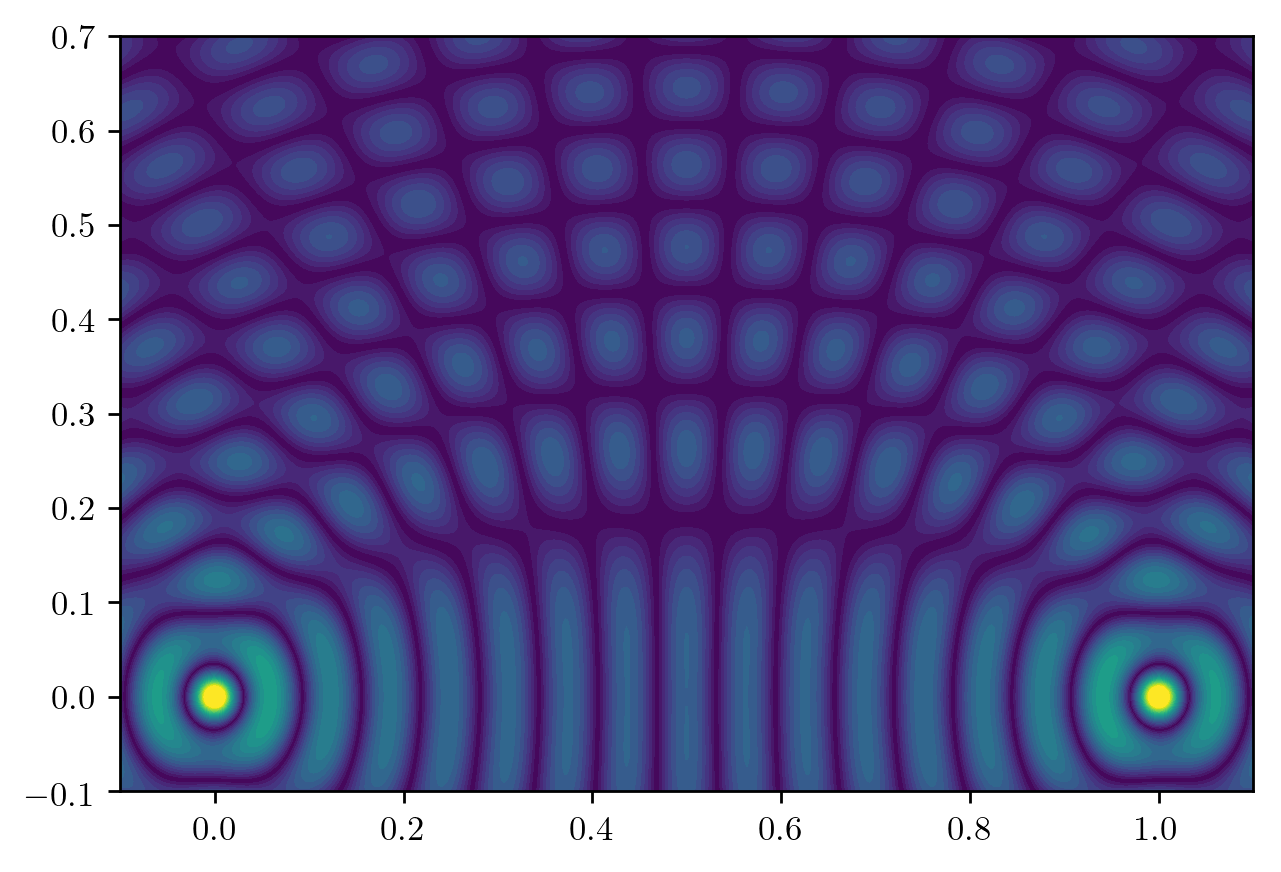
\includegraphics[width=0.4\columnwidth]{img/3_projet_enseignement/interf_cylindriques}
\end{frame}

\begin{frame}{Bonus : vulgarisation en L1-L2}
Inspiration : UE \emph{Culture biologie numérique} à l'Université Paris Diderot.

Vulgarisation d'un thème de L1-L2 via un \textbf{article de blog} et un oral (cf ``physics show'' d'Orsay).

\begin{columns}
\begin{column}{0.6\textwidth}
\begin{block}{Objectifs :}
	\begin{itemize}
		\item Réappropriation des notions,
		\item Travail en groupe,
		\item Projet,
		\item Découverte de la vulgarisation.
	\end{itemize}
\end{block}
\end{column}
\begin{column}{0.4\textwidth}
\centering
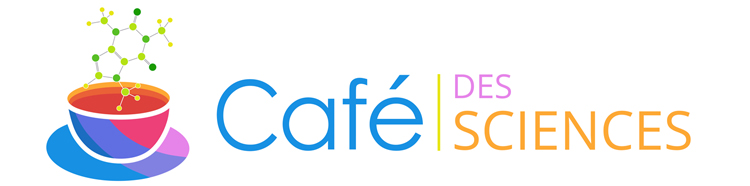
\includegraphics[width=\columnwidth]{img/3_projet_enseignement/banniere-cafe-big6}
\end{column}
\end{columns}
\end{frame}